\documentclass[8pt,a4paper,compress,handout]{beamer}

\usepackage{/home/siyer/lib/slides}

\title{Case Study: $N$-Body Problem}
\date{}

\begin{document}
\begin{frame}
\vfill
\titlepage
\end{frame}

\begin{frame}
\frametitle{Outline}
\tableofcontents
\end{frame}

\section{$N$-Body Simulation}
\begin{frame}[fragile]
Newton's first law of motion states that a body in motion remains in motion at the same velocity unless acted on by an outside force. 

\bigskip

Newton's second law of motion explains how outside forces on a body affect its velocity.

\bigskip

The $N$-body simulation problem, originally formulated by Isaac Newton over 350 years ago, describes the motion of the $N$ bodies, mutually affected by gravitational forces.
\end{frame}

\section{Body Data Type}
\begin{frame}[fragile]
A data type \lstinline{Body} for moving bodies:
\begin{center}
\begin{tabular}{cc}
method & description \\ \hline
\lstinline$Body(r, v, mass)$ & a new body $b$ with mass $mass$ at position $r$ moving at velocity $v$ \\
\lstinline$b.move(f, dt)$ & move $b$ by applying force $f$ for $dt$ seconds \\
\lstinline$b.forceFrom(a)$ & force vector from body $a$ on body $b$ \\
\lstinline$b.draw()$ & draw body $b$ to standard draw
\end{tabular} 
\end{center}

\bigskip

Note that \lstinline{Body} is a \lstinline{Vector} client --- the values of the data type are \lstinline{Vector} objects that carry the body's position and velocity, as well as a float that carries the mass.

\bigskip

We use Newton's second law ($\mathbf{F}=m\mathbf{a}$) for updating the position and velocity of a body due to a given force vector \lstinline{f} and amount of time \lstinline{dt}.
\begin{lstlisting}[language=Python]
a = f.scale(1.0 / mass)
v = v + a.scale(dt)
r = r + v.scale(dt)
\end{lstlisting}

\begin{center}
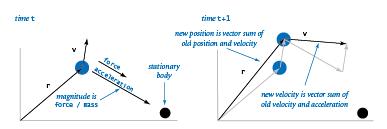
\includegraphics[scale=0.45]{figures/vector_add_acc.png}

\smallskip

\tiny Motion near a stationary body
\end{center}
\end{frame}

\begin{frame}[fragile]
We use Newton's law of universal gravitation ($\mathbf{F}=G\frac{m_1m_2}{r^2}\hat{\mathbf{r}}$) for computing the force imposed on one body by another.

\begin{lstlisting}[language=Python]
G = 6.67e-11
delta = a._r - b._r
dist = abs(delta)
magnitude = G * a._mass * b._mass / (dist * dist)
f = delta.direction().scale(magnitude)
\end{lstlisting}

\begin{center}
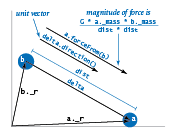
\includegraphics[scale=0.5]{figures/vector_force.png}

\smallskip

\tiny Force on one body due to another
\end{center}
\end{frame}

\begin{frame}[fragile]
\begin{framed}
\tiny \lstinline{body.py}: Defines a data type \lstinline{Body} representing a gravitating body.
\end{framed}

\begin{lstlisting}[language=Python]
import stddraw

class Body:
    def __init__(self, r, v, mass):
        self._r = r
        self._v = v
        self._mass = mass

    def move(self, f, dt):
        a = f.scale(1 / self._mass)
        self._v = self._v + (a.scale(dt))
        self._r = self._r + self._v.scale(dt)

    def forceFrom(self, other):
        G = 6.67e-11
        delta = other._r - self._r
        dist = abs(delta)
        magnitude = (G * self._mass * other._mass) / (dist * dist)
        return delta.direction().scale(magnitude)

    def draw(self):
        stddraw.setPenRadius(0.0125)
        stddraw.point(self._r[0], self._r[1])
\end{lstlisting}
\end{frame}

\section{Universe Data Type}
\begin{frame}[fragile]
The data type \lstinline{Universe} models the universe:
\begin{center}
\begin{tabular}{cc}
method & description \\ \hline
\lstinline$Universe(file)$ & a new universe $u$ built from a description in $file$ \\
\lstinline$u.increaseTime(dt)$ & update $u$ by simulating the universe for $dt$ seconds \\
\lstinline$u.draw()$ & draw universe $u$ to standard draw
\end{tabular} 
\end{center}

\bigskip

The constructor reads the universe parameters and body descriptions from a file that contains the following information:
\begin{itemize}
\item The number of bodies.
\item The radius of the universe.
\item The position, velocity, and mass of each body.
\end{itemize}
\begin{lstlisting}[language={}]
$ more 2body.txt
2 
5.0e10 
0.0e00  4.5e10  1.0e04 0.0e00 1.5e30 
0.0e00 -4.5e10 -1.0e04 0.0e00 1.5e30 
\end{lstlisting}
\end{frame}

\begin{frame}[fragile]
\begin{framed}
\tiny \lstinline{universe.py}: Accepts a string \carg{filename} and a float \carg{dt} as command-line arguments, and simulates the motion in the universe defined by the contents of \carg{filename}, increasing time at the rate specified by \carg{dt}.
\end{framed}

\begin{lstlisting}[language=Python]
import stdarray
import stddraw
import sys
from body import Body 
from instream import InStream
from vector import Vector

class Universe:
    def __init__(self, filename):
        instream = InStream(filename)
        n = instream.readInt()
        radius = instream.readFloat()
        stddraw.setXscale(-radius, +radius)
        stddraw.setYscale(-radius, +radius)
        self._bodies = stdarray.create1D(n)
        for i in range(n):
            rx   = instream.readFloat()
            ry   = instream.readFloat()
            vx   = instream.readFloat()
            vy   = instream.readFloat()
            mass = instream.readFloat()
            r = Vector([rx, ry])
            v = Vector([vx, vy])
            self._bodies[i] = Body(r, v, mass)
\end{lstlisting}
\end{frame}

\begin{frame}[fragile]
\begin{lstlisting}[language=Python]
    def increaseTime(self, dt):
        n = len(self._bodies)
        f = stdarray.create1D(n, Vector([0, 0]))
        for i in range(n):
            for j in range(n):
                if i != j:
                    bodyi = self._bodies[i]
                    bodyj = self._bodies[j]
                    f[i] = f[i] + bodyi.forceFrom(bodyj)
        for i in range(n):
            self._bodies[i].move(f[i], dt)    

    def draw(self):
        for body in self._bodies:
            body.draw()

def main():
    filename = sys.argv[1]
    dt = float(sys.argv[2])
    universe = Universe(filename)
    while True:
        universe.increaseTime(dt)
        stddraw.clear()
        universe.draw()
        stddraw.show(10)

if __name__ == '__main__':
    main()
\end{lstlisting}
\end{frame}

\begin{frame}[fragile]
\begin{minipage}{200pt}
2-body system:
\begin{lstlisting}[language={}]
$ more 2body.txt
2 
5.0e10 
0.0e00  4.5e10  1.0e04 0.0e00 1.5e30 
0.0e00 -4.5e10 -1.0e04 0.0e00 1.5e30 
$ python universe.py 2body.txt 20000
\end{lstlisting}

\bigskip

3-body system:
\begin{lstlisting}[language={}]
$ more 3body.txt
3 
1.25e11 
0.0e00  0.0e00 0.05e04 0.0e00 5.97e24 
0.0e00  4.5e10  3.0e04 0.0e00 1.989e30 
0.0e00 -4.5e10 -3.0e04 0.0e00 1.989e30 
$ python universe.py 3body.txt 20000
\end{lstlisting}

\bigskip

4-body system:
\begin{lstlisting}[language={}]
$ more 4body.txt
4 
5.0e10 
-3.5e10 0.0e00 0.0e00  1.4e03 3.0e28 
-1.0e10 0.0e00 0.0e00  1.4e04 3.0e28 
 1.0e10 0.0e00 0.0e00 -1.4e04 3.0e28 
 3.5e10 0.0e00 0.0e00 -1.4e03 3.0e28 
$ python universe.py 4body.txt 20000
\end{lstlisting}
\end{minipage}%
\hfill
\begin{minipage}{100pt}
\begin{center}
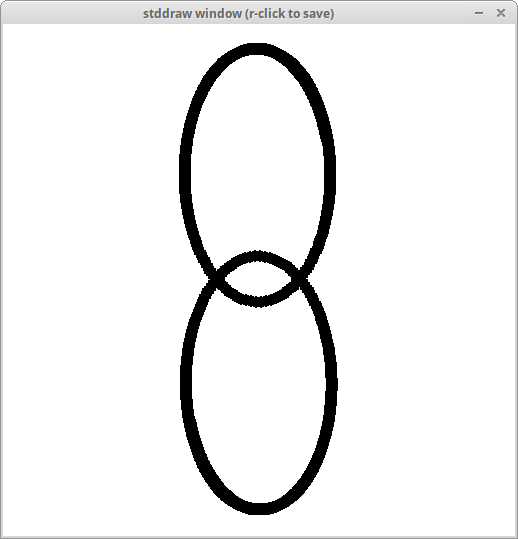
\includegraphics[scale=0.13]{figures/2body.png}

\smallskip

\tiny 2-body system

\smallskip

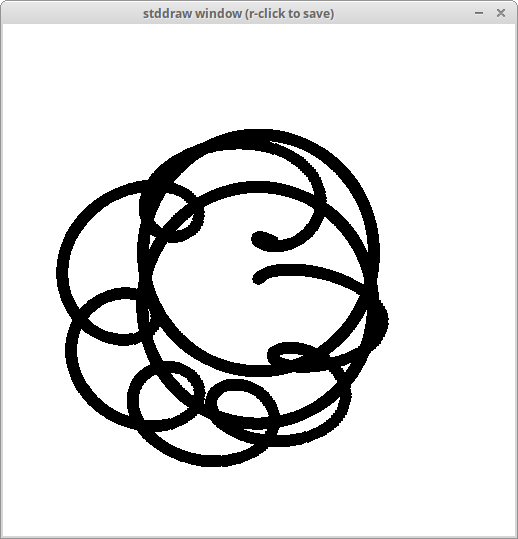
\includegraphics[scale=0.13]{figures/3body.png}

\smallskip

\tiny 3-body system

\smallskip

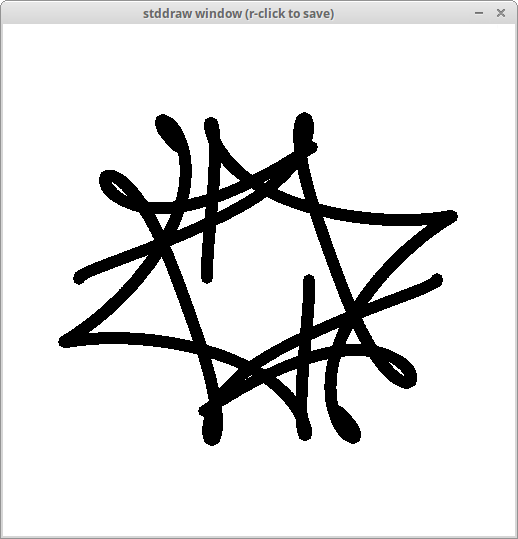
\includegraphics[scale=0.13]{figures/4body.png}

\smallskip

\tiny 4-body system
\end{center}
\end{minipage}
\end{frame}

\end{document}
